\documentclass{article}
\usepackage{cite}

\usepackage{titlesec}
\setcounter{secnumdepth}{4}

\usepackage{amsmath}

\usepackage{graphicx}
\graphicspath{{./figures/}}

\title{Data Analysis for Predictive Maintenance of a Straightening Machine in the Steel Industry}
\date{2023-XX-XX}
\author{Paul Barron}
\begin{document}
\pagenumbering{gobble}
\maketitle
\newpage
\pagenumbering{arabic}
\tableofcontents
\newpage
\section{Abstract}
 
\newpage
\section{Introduction}

Understand what signals are related to each other
Understand signals from a statistical point of view
Identify which features are the important ones and which are not of interest

\newpage  
\section{Literature Review}
Condition monitoring.\\
Reference ~\cite{caesarendra2017review}.\\
Reference ~\cite{james2013introduction}.\\
Reference ~\cite{soualhi2021novel}.

\newpage  
\section{Methodology}
Preprocessing: you could standardize the signals, eliminate the dc-offset, … before calculating the features.
Calculate features of the different signals, i.e., correlations between raw signals, kurtosis, mean, skewness, …,
Verify features which are extracted from the diagnostic feature extraction toolbox, i.e., what it is kurtosis, THD,… for the toolbox. You can compare the results given by the matlab function and the toolbox. Important to look at the formula which is given on the help description of the function.

Compute correlations between 2 features.
Calculate a in X1 = aX2, where X1 and X2 represents the features.
Calculate R2, which relates to the variance in linear regression models.
Plot some of the regression models between 2 features which are highly correlated where X1 is one axis, and X2 is the other axis. Do not plot all of them.

Compute a multivariable regression model.
Guide yourself by eliminating features which are highly correlated between each other by using the info you got in the previous part where you compute correlations between 2 features.

\subsection{Pre processing (state detection)}
The state detection for this application will be performed using one signal in particular, 

\subsection{Feature Extraction}


\subsection{Statistical analysis}
$$ AIC = 2k - 2Ln(L) $$  
$$ nAIC = log $$
 
\subsection{Time Domain Features} 	
Features in the time domain.
\subsection{Statistical Features}
\subsubsection{Mean}
$$ \bar{x} = \frac{\sum^N_{i=i} x_i}{N} $$
\subsubsection{Standard Deviation}  
$$ Var =\frac{\sum^N_{i=1}(x_i-m)^2}{(N-1)\sigma^2} $$
\subsubsection{Root Mean Square (RMS)}
$$ RMS = \sqrt{\frac{1}{N} \sum^N_{i=1}x^2_i} $$
\subsubsection{Shape Factor}
$$ \frac{ \sqrt{\frac{1}{N} \sum^N_{i=1}x_i^2} }  {\frac{1}{N}\sum^N_{i=1}|x_i|} $$
\subsubsection{Kurtosis} 
$$ Ku = \frac{\sum^N_{i=1}(x_i-m)^4)}{(N-1)\sigma^4} $$ 
\subsubsection{Skewness} 
$$ Sk = \frac{\sum^2_{i=1}(x_i-m)^3}{(N-1)\sigma^3} $$
  
\subsection{Impulsive Metrics}  
\subsubsection{Peak Value}
$$ PV = max(x_i) $$ 
\subsubsection{Impulse Factor} 
$$ x_{clear} = \frac{x_p}{(\frac{1}{N}\sum^N_{i=1}|x_i|)} $$  
\subsubsection{Crest Factor} 
$$ CF = \frac{max|x_i|}{\sqrt{\frac{1}{N}}\sum^N_{i=1}x^2_i} $$
\subsubsection{Clearance Factor} 
$$ x_{clear} = \frac{x_p}{(\frac{1}{N}\sum^N_{i=1}\sqrt{|x_i|)^2}} $$
  
\subsubsection{Signal Processing Metrics}
\subsubsection{Signal to Noise Ratio (SNR)} 
\subsubsection{Signal-to-Noise And Distortion (SINAD)} 
\subsubsection{Total Harmonic Distortion (THD)}   

\subsubsection{Frequency Domain Features}
Features in the frequency domain.
\subsubsection{Band Power}
\subsubsection{Peak Amplitude}
\subsubsection{Peak Frequency}

\newpage  
\section{Results}
Figure \ref{fig:StateDetection} shows the pulses that were identified for from each file. Two files contained no identified pulses. In total 240(?) pulses were identified to extract features from in the next stage.

\begin{figure}[h!]
    \centering
    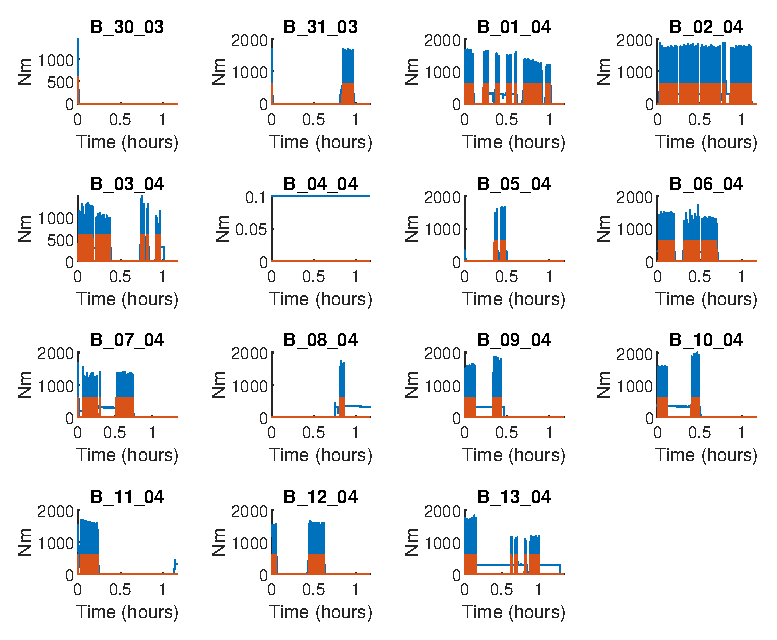
\includegraphics{figures/StateDetectionFig.eps}
    \caption{State detection signal vs 21:20 Actual moment under Rollers}
    \label{fig:StateDetection}
\end{figure}

\newpage  
\section{Conclusion}

\newpage 
\section{Discussion} 

\newpage  
\section{References} 
\bibliography{References}
\bibliographystyle{plain} 

\newpage  
\section{Appendix A}

\end{document}